\documentclass[aspectratio=169]{beamer}
\usepackage{graphicx}
\usepackage{xcolor}
\usepackage{pgfpages}
\usepackage{tikz}
\usepackage[european]{circuitikz}
\usetikzlibrary{arrows.meta,positioning,calc}

% Slightly tighter global line spacing for compact slide blocks.
\linespread{0.92}

% Beamer supports presenter notes via \note{...}.
% Default build hides notes. For presenter notes, change this to e.g.:
%   \setbeameroption{show notes on second screen=right}
\setbeameroption{hide notes}

% Nord-inspired slide colors
\definecolor{NordBody}{HTML}{4C566A}
\definecolor{NordBlue}{HTML}{5E81AC}
\definecolor{NordRed}{HTML}{BF616A}
\definecolor{NordGreen}{HTML}{A3BE8C}
\definecolor{NordOrange}{HTML}{D08770}
\definecolor{NordPurple}{HTML}{B48EAD}
\definecolor{NordPanel}{HTML}{ECEFF4}

% Reusable flow-diagram layout settings.
\newcommand{\FlowTitleGap}{0.7ex}
\newcommand{\FlowTitle}[1]{{\raggedright\scriptsize #1\par}\vspace{\FlowTitleGap}}
\newcommand{\FlowCodeFont}{\ttfamily\fontsize{5.4}{5.5}\selectfont\color{black}}
\newcommand{\FlowCodeBlock}[2]{{#1\renewcommand{\arraystretch}{0.82}\begin{tabular}{@{}l@{}}#2\end{tabular}}}
\newcommand{\FlowLeftX}{0.05}
\newcommand{\FlowMidX}{0.30}
\newcommand{\FlowTemplateX}{0.24}
\newcommand{\FlowOutputX}{0.67}
\newcommand{\FlowParamW}{0.11\linewidth}
\newcommand{\FlowInputW}{0.16\linewidth}
\newcommand{\FlowInputSchematicW}{0.32\linewidth}
\newcommand{\FlowEngineW}{0.25\linewidth}
\newcommand{\FlowTemplateW}{0.34\linewidth}
\newcommand{\FlowOutputW}{0.30\linewidth}
\newcommand{\FlowSchematicImgW}{0.90\linewidth}
\newcommand{\FlowSmallSchematicImgW}{0.82\linewidth}
\newcommand{\FlowEdgeLow}{0.333}
\newcommand{\FlowEdgeHigh}{0.667}
\tikzset{
  flowdiagram/.style={x=\linewidth, y=1cm, font=\scriptsize},
  flowinput/.style={draw=NordGreen!80!black, rounded corners=2pt, line width=0.8pt, fill=NordGreen!16, align=left, inner sep=6pt},
  flowengine/.style={draw=NordRed!85!black, rounded corners=2pt, line width=0.8pt, fill=NordRed!12, align=left, inner sep=6pt},
  flowartifact/.style={draw=NordBlue!85!black, rounded corners=2pt, line width=0.7pt, fill=NordBlue!7, align=left, inner sep=7pt},
  flowarrow/.style={-{Stealth[length=3mm]}, line width=0.8pt, draw=NordBody},
}

% Custom footline with slide numbers in bottom left
\setbeamertemplate{footline}{
  \hspace{1em}%
  \usebeamercolor[fg]{page number in head/foot}%
  \usebeamerfont{page number in head/foot}%
  \insertframenumber\,/\,\inserttotalframenumber%
  \vskip2pt%
}

\beamertemplatenavigationsymbolsempty

% Text-color theme
\setbeamercolor{normal text}{fg=NordBody}
\setbeamercolor{title}{fg=NordBlue}
\setbeamercolor{frametitle}{fg=NordBlue}
\setbeamercolor{structure}{fg=NordBlue}
\setbeamercolor{itemize/enumerate body}{fg=NordBody}
\setbeamercolor{itemize/enumerate subbody}{fg=NordBody}
\setbeamercolor{itemize/enumerate subsubbody}{fg=NordBody}
\setbeamercolor{itemize item}{fg=NordBlue}
\setbeamercolor{itemize subitem}{fg=NordBlue}
\setbeamercolor{itemize subsubitem}{fg=NordBlue}
\setbeamercolor{enumerate item}{fg=NordBlue}
\setbeamercolor{enumerate subitem}{fg=NordBlue}
\setbeamercolor{enumerate subsubitem}{fg=NordBlue}

% Global hyperlink style
\hypersetup{
  colorlinks=true,
  allcolors=NordBlue
}

\title{Programmatic analog IC design\\{\large without reinventing the wheel}}
\author{Kennedy Caisley}
\institute{University of Bonn}
\date{FSiC 2026, 7 July 2026}

\begin{document}

%% ============================================================
%% Title
%% ============================================================
\begin{frame}
  \titlepage
  \vfill
  \begin{center}
    
\includegraphics[height=1.3cm]{images/logo_bonn.jpg}%
    \hspace{0.8cm}%
    
\includegraphics[height=1.3cm]{images/logo_ftd.jpg}%
    \hspace{0.8cm}%
    
\includegraphics[height=1.43cm]{images/logo_silab.png}%
  \end{center}
  \note{\begin{itemize}
    \item PhD student.
    \item Share thoughts on using general-purpose programming languages to author analog and mixed-signal circuit designs.
  \end{itemize}}
\end{frame}



%% ============================================================
%% Motivation
%% ============================================================
\begin{frame}
  \frametitle{Motivation: CMOS image sensors}
  \begin{center}
    
\includegraphics[height=0.78\textheight]{images/arch.pdf}
  \end{center}
  \note{\begin{itemize}
    \item CMOS image sensors are large arrays of repeated structures.
    \item Most blocks are roughly square, and exact geometry is less critical than in RF design.
    \item Small area improvements scale across the array.
    \item There are many design variations worth exploring.
  \end{itemize}}
\end{frame}

\begin{frame}
  \frametitle{A sad (far too frequent) story}
  \begin{center}
  \begin{tikzpicture}[
    terminal/.style={draw=NordBody, rounded corners=4pt, line width=0.9pt, fill=NordBody!7, inner sep=0pt},
    titlebar/.style={fill=NordBody, rounded corners=4pt},
    control/.style={circle, minimum size=6pt, inner sep=0pt},
    termtext/.style={font=\ttfamily\scriptsize, text=black, anchor=north west},
  ]
    \node[terminal, minimum width=0.78\linewidth, minimum height=0.58\textheight, anchor=north west] (term) at (0,0) {};
    \path[titlebar] (term.north west) rectangle ([yshift=-0.50cm]term.north east);
    \fill[NordRed]    ([xshift=0.28cm,yshift=-0.25cm]term.north west) circle[radius=3pt];
    \fill[NordOrange] ([xshift=0.52cm,yshift=-0.25cm]term.north west) circle[radius=3pt];
    \fill[NordGreen]  ([xshift=0.76cm,yshift=-0.25cm]term.north west) circle[radius=3pt];
    \node[font=\ttfamily\scriptsize, text=white, anchor=west] at ([xshift=1.05cm,yshift=-0.25cm]term.north west) {kennedy@frida:/design/netlists};

    \node[termtext] at ([xshift=0.40cm,yshift=-0.78cm]term.north west) {\begin{tabular}{@{}lll@{}}
      \multicolumn{3}{@{}l@{}}{\textcolor{NordGreen!55!black}{\$} ls -lht}\\[1pt]
      \textcolor{NordBody}{date} & \textcolor{NordBody}{size} & \textcolor{NordBody}{name}\\
      Jun 12 18:31 & 18K & preamp.sp\\
      Jun 13 00:07 & 19K & preamp\_v2.sp\\
      Jun 13 03:42 & 22K & preamp\_v3.sp\\
      Jun 13 03:55 & 22K & preamp\_v3a.sp\\
      Jun 13 04:11 & 21K & preamp\_v3\_edit.sp\\
      Jun 13 04:58 & 24K & preamp\_final.sp\\
      Jun 13 05:03 & 24K & preamp\_final\_final.sp\\
      Jun 13 05:07 & 25K & preamp\_final\_final2.sp\\
      Jun 13 05:12 & 17K & preamp\_oops\_made\_a\_mistake.sp\\
      Jun 13 05:29 & 26K & preamp\_actually\_use\_this\_one.sp
    \end{tabular}};
  \end{tikzpicture}
  \end{center}
  \note{\begin{itemize}
    \item There is a large potential for reuse.
    \item Reuse can be ruined by differences between PDKs.
    \item It can also be lost when design exploration is not recorded.
    \item Graphical schematic workflows make this especially hard to preserve.
  \end{itemize}}
\end{frame}

\begin{frame}
  \frametitle{What happens when we design with code?}
  \vfill
  \begin{center}
  \begin{minipage}{0.88\textwidth}
  \begin{columns}[T,totalwidth=\textwidth]
    \begin{column}{0.45\textwidth}
      \textcolor{NordGreen!55!black}{\large Pros}
      \vspace{0.5em}
      \begin{itemize}
        \item[\textcolor{NordGreen!65!black}{\Large $\checkmark$}] Revision control in plaintext
        \item[\textcolor{NordGreen!65!black}{\Large $\checkmark$}] Easier collaborative work
        \item[\textcolor{NordGreen!65!black}{\Large $\checkmark$}] More reproducible workflows*
        \item[\textcolor{NordGreen!65!black}{\Large $\checkmark$}] Design changes faster
        \item[\textcolor{NordGreen!65!black}{\Large $\checkmark$}] Sweep many design options
      \end{itemize}
    \end{column}
    \hfill
    \begin{column}{0.45\textwidth}
      \textcolor{NordRed!85!black}{\large Cons}
      \vspace{0.5em}
      \begin{itemize}
        \item[\textcolor{NordRed!85!black}{\Large $\checkmark$}] Code is an additional and unfamiliar abstraction
        \item[\textcolor{NordRed!85!black}{\Large $\checkmark$}] Netlists poorly show intent
        \item[\textcolor{NordRed!85!black}{\Large $\checkmark$}] Connectivity mistakes difficult to catch
        \item[\textcolor{NordRed!85!black}{\Large $\checkmark$}] Initial design is very slow
      \end{itemize}
    \end{column}
  \end{columns}
  \end{minipage}
  \end{center}
  \vfill
  \note{\begin{itemize}
    \item Benefits: revision control and easier collaborative work in plaintext.
    \item Reproducibility of the workflow, at least sometimes.
    \item Design changes become faster once the abstraction exists.
    \item Easy to try multiple options; even experienced designers want this.
    \item Cons: code is an additional and unfamiliar abstraction.
    \item Digital designers have Verilog; analog designers have little beyond netlists, which poorly show design intent.
    \item Connectivity mistakes are difficult to catch.
    \item Initial design is very slow, regardless of skill level.
  \end{itemize}}
\end{frame}

\begin{frame}
  \frametitle{Scope: Netlists, Tests, \& Layouts}
  \begin{center}
  \begin{columns}[c,totalwidth=0.95\textwidth]
    \begin{column}{0.50\textwidth}
      \centering
      {\normalsize\textcolor{NordBody}{From system arch\ldots}\par}\vspace{0.8ex}
      
\includegraphics[width=\linewidth]{images/adc_block.pdf}
    \end{column}
    \begin{column}{0.05\textwidth}
      \centering
      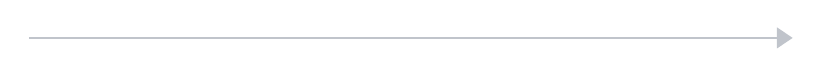
\begin{tikzpicture}[x=\linewidth,y=1cm]
        \draw[-{Triangle[length=2mm,width=2.6mm]}, line width=0.9pt, draw=NordBody!35] (0.10,0) -- (0.90,0);
      \end{tikzpicture}
    \end{column}
    \begin{column}{0.40\textwidth}
      \centering
      {\normalsize\textcolor{NordBody}{\ldots to GDS}\par}\vspace{0.8ex}
      
\includegraphics[width=\linewidth,height=0.66\textheight,keepaspectratio]{images/frida_adc.png}
    \end{column}
  \end{columns}

  \vspace{1.4ex}
  {\normalsize\textcolor{NordBody}{Pragmatic constraint: No new tools; just combine existing code-based options}}
  \end{center}
  \note{\begin{itemize}
    \item I build this ADC for image-sensor readout.
    \item Start with the ADC block diagram and show how it becomes an implemented layout.
    \item Focus briefly on behavioral modeling.
    \item Then focus on netlist authoring.
    \item Then testbench creation, SPICE simulation, and analysis: testbench diagrams, HDL21-to-plotting flow, and a small ADC non-linearity plot.
    \item Finish with layout.
  \end{itemize}}
\end{frame}

\begin{frame}
  \frametitle{A word on modeling}
  \begin{center}
  \begin{tikzpicture}
    \node[flowartifact, text width=0.96\linewidth, inner sep=7pt] {
      {\raggedright\scriptsize\ttfamily \$ python adc\_model.py\par}\vspace{0.7ex}
      {\centering
\includegraphics[width=0.94\linewidth,height=0.64\textheight,keepaspectratio]{images/adc_discrete_model.pdf}\par}
    };
  \end{tikzpicture}
  \end{center}
  \note{\begin{itemize}
    \item Before designing, it is very helpful to make a model with behavioral accuracy.
    \item MATLAB or Verilog-A are common choices.
    \item Make sure the model is essentially a linear time-invariant system with a clear order of calculation.
    \item Record waveforms to a standard time-step model.
    \item Do not overdo it, because you likely will not be able to build half the blocks anyway.
    \item Use this mainly for convergence.
    \item With Verilog-A support, you can do this inside the simulator too.
    \item I had access to that flow, but found Python more ergonomic despite the disadvantage of not being integrated.
  \end{itemize}}
\end{frame}

%% ============================================================
%% Netlist generation
%% ============================================================
\begin{frame}
  \frametitle{Netlisting: Traditional schematic}
  \begin{center}
  \begin{tikzpicture}[flowdiagram]
    \node[flowinput, text width=\FlowInputSchematicW, anchor=west] (schem_in) at (0.13,0) {
      \FlowTitle{Schematic}
      {\centering
\includegraphics[width=\FlowSchematicImgW]{images/preamp_test.pdf}\par}
    };

    \node[flowartifact, text width=\FlowOutputW, anchor=west] (net_out) at (0.55,0) {
      \FlowTitle{Netlist}
      \FlowCodeBlock{\FlowCodeFont}{
        .subckt preamp inn inp clk xp xn\\
        MP1 xp clk vdd vdd pch w=120n l=100n\\
        MP2 xn clk vdd vdd pch w=120n l=100n\\
        MN1 xp inn nsrc vss nch w=480n l=100n\\
        MN2 xn inp nsrc vss nch w=480n l=100n\\
        MN3 nsrc clk vss vss nch w=240n l=200n\\
        .ends preamp
      }
    };

    \draw[flowarrow] (schem_in.east) -- (net_out.west);
  \end{tikzpicture}
  \end{center}
  \note{\begin{itemize}
    \item Goal: text-based netlist generation with multi-PDK support.
    \item Parameterize topology, device flavor, and sizing using lambda-style dimensions.
    \item Tools tried: pure SPICE netlists, spicelib, PySpice, HDL21, and BAG3.
    \item These mostly fall into the generator-based automation family.
    \item Limitation: no useful GUI; Cadence spice-in and Graphviz-to-netlistsvg are not very tenable.
  \end{itemize}}
\end{frame}

\begin{frame}
  \frametitle{Netlisting: Manual writing w/ parameters}
  \begin{center}
  \begin{tikzpicture}[flowdiagram]
    \node[flowinput, text width=\FlowParamW, anchor=west] (params) at (\FlowLeftX,0) {
      \FlowTitle{Params}
      \FlowCodeBlock{\FlowCodeFont}{
        \textcolor{NordBlue}{win}=8\\
        \textcolor{NordBlue}{wtop}=2\\
        \textcolor{NordBlue}{wtail}=4\\
        \textcolor{NordBlue}{ltail}=2
      }
    };

    \node[flowengine, text width=\FlowTemplateW, anchor=west] (tmpl) at (\FlowTemplateX,0) {
      \FlowTitle{Parameterized netlist}
      \FlowCodeBlock{\FlowCodeFont}{
        .subckt preamp inn inp clk xp xn\\
        .param \textcolor{NordBlue}{win}=8 \textcolor{NordBlue}{wtop}=2 \textcolor{NordBlue}{wtail}=4 \textcolor{NordBlue}{ltail}=2\\
        MP1 xp clk vdd vdd pch w=\textcolor{NordBlue}{wtop}*60n l=100n\\
        MP2 xn clk vdd vdd pch w=\textcolor{NordBlue}{wtop}*60n l=100n\\
        MN1 xp inn nsrc vss nch w=\textcolor{NordBlue}{win}*60n l=100n\\
        MN2 xn inp nsrc vss nch w=\textcolor{NordBlue}{win}*60n l=100n\\
        MN3 nsrc clk vss vss nch w=\textcolor{NordBlue}{wtail}*60n l=\textcolor{NordBlue}{ltail}*100n\\
        .ends preamp
      }
    };

    \node[flowartifact, text width=\FlowOutputW, anchor=west] (spice) at (\FlowOutputX,1.25) {
      \FlowTitle{Netlist}
      \FlowCodeBlock{\FlowCodeFont}{
        .subckt preamp inn inp clk xp xn\\
        MP1 xp clk vdd vdd pch w=120n l=100n\\
        MP2 xn clk vdd vdd pch w=120n l=100n\\
        MN1 xp inn nsrc vss nch w=480n l=100n\\
        MN2 xn inp nsrc vss nch w=480n l=100n\\
        MN3 nsrc clk vss vss nch w=240n l=200n\\
        .ends preamp
      }
    };

    \node[flowartifact, text width=\FlowOutputW, anchor=west] (schem) at (\FlowOutputX,-1.75) {
      \FlowTitle{Schematic}
      {\centering
\includegraphics[width=\FlowSmallSchematicImgW]{images/preamp_test.pdf}\par}
    };

    \draw[flowarrow] (params.east) -- (tmpl.west);
    \draw[flowarrow] ($(tmpl.south east)!\FlowEdgeHigh!(tmpl.north east)$) -- ++(0.02,0) |- (spice.west);
    \draw[flowarrow] ($(tmpl.south east)!\FlowEdgeLow!(tmpl.north east)$) -- ++(0.02,0) |- (schem.west);
  \end{tikzpicture}
  \end{center}
  \begin{tikzpicture}[remember picture, overlay]
    \node[anchor=south west, text width=0.28\linewidth, align=right, text=NordBody]
      at ([xshift=0.55cm,yshift=0.63cm]current page.south west) {
        \scriptsize Tip: {\setlength{\fboxsep}{1.2pt}\colorbox{NordPanel}{\texttt{netlistsvg}}} is the best existing option for automatic schematic visualization
      };
    \node[anchor=south west, inner sep=0pt]
      at ([xshift=4.75cm,yshift=0.25cm]current page.south west) {
        
\includegraphics[height=3.48cm,keepaspectratio]{images/preamp_netlistsvg.pdf}
      };
  \end{tikzpicture}
  \note{\begin{itemize}
    \item Graphical schematics or raw netlists allow parameterization of device dimensions or supply voltages.
    \item Topology, device type, and PDK are still effectively fixed.
    \item Module substitution and varying port count are not possible in a useful procedural way.
  \end{itemize}}
\end{frame}

\begin{frame}
  \frametitle{Netlisting: Procedural generation}
  \begin{center}
  \begin{tikzpicture}[flowdiagram]
    \node[flowinput, text width=\FlowInputW, anchor=west] (params) at (\FlowLeftX,0.95) {
      \FlowTitle{Params}
      \FlowCodeBlock{\FlowCodeFont}{
        [\textcolor{NordBlue}{win}=8, \textcolor{NordBlue}{wtop}=2,\\
        \textcolor{NordBlue}{wtail}=4, \textcolor{NordBlue}{ltail}=2,\\
        \textcolor{NordBlue}{topo\_in}=nmos,\\
        \textcolor{NordBlue}{topo\_pow}=dyn,\\
        \textcolor{NordBlue}{tech}=65,\\
        \textcolor{NordBlue}{format}=spice]
      }
    };
    \node[flowinput, text width=\FlowInputW, anchor=west] (tech) at (\FlowLeftX,-1.15) {
      \FlowTitle{PDK}
      \FlowCodeBlock{\FlowCodeFont}{
        SPICE deck\\
        device flavors\\
        \textcolor{NordGreen!55!black}{$\lambda$-dimensions}
      }
    };

    \node[flowengine, text width=\FlowEngineW, anchor=west] (gen) at (\FlowMidX,0) {
      \FlowTitle{Generator (e.g. Hdl21)}
      \FlowCodeBlock{\FlowCodeFont}{
        \textcolor{NordBlue}{def} build\_preamp(module, param):\\
        \ \ \textcolor{NordBody}{[...impl...]}\\
        \ \ \textcolor{NordPurple}{return} module
      }
    };

    \node[flowartifact, text width=\FlowOutputW, anchor=west] (spice) at (\FlowOutputX,1.25) {
      \FlowTitle{Netlist}
      \FlowCodeBlock{\FlowCodeFont}{
        .subckt preamp inn inp clk xp xn\\
        MP1 xp clk vdd vdd pch w=120n l=100n\\
        MP2 xn clk vdd vdd pch w=120n l=100n\\
        MN1 xp inn nsrc vss nch w=480n l=100n\\
        MN2 xn inp nsrc vss nch w=480n l=100n\\
        MN3 nsrc clk vss vss nch w=240n l=200n\\
        .ends preamp
      }
    };
    \node[flowartifact, text width=\FlowOutputW, anchor=west] (schem) at (\FlowOutputX,-1.75) {
      \FlowTitle{Schematic}
      {\centering
\includegraphics[width=\FlowSmallSchematicImgW]{images/preamp_test.pdf}\par}
    };

    \draw[flowarrow] (params.east) -- ++(0.025,0) |- ($(gen.south west)!\FlowEdgeHigh!(gen.north west)$);
    \draw[flowarrow] (tech.east) -- ++(0.025,0) |- ($(gen.south west)!\FlowEdgeLow!(gen.north west)$);
    \draw[flowarrow] ($(gen.south east)!\FlowEdgeHigh!(gen.north east)$) -- ++(0.035,0) |- (spice.west);
    \draw[flowarrow] ($(gen.south east)!\FlowEdgeLow!(gen.north east)$) -- ++(0.035,0) |- (schem.west);
  \end{tikzpicture}
  \end{center}
  \begin{tikzpicture}[remember picture, overlay]
    \node[anchor=south, text width=0.88\linewidth, align=center, text=NordBody]
      at ([yshift=0.34cm]current page.south) {
        \scriptsize Tip: Some tools for netlist generation include Hdl21 \href{https://wiki.f-si.org/index.php?title=Open_(and_Closed)_Source_Analog_Design_with_Hdl21_\%26_VLSIR}{[FSiC 23]},\\
        Substrate \href{https://fossi-foundation.org/latch-up/2026\#substrate-a-statically-typed-framework-for-designing-highly-configurable-analog-and-mixed-signal-circuit-generators}{[Latch-Up 26]}, BAG \href{https://doi.org/10.1109/OJCAS.2024.3502641}{[OJCAS 25]}, and ORDec \href{https://wiki.f-si.org/index.php?title=ORDeC:_Progress_in_text-driven_analog_IC_design_from_schematic_to_layout}{[FSiC 26]}.
      };

  \end{tikzpicture}
  \note{\begin{itemize}
    \item A general-purpose programming language plus a library of primitives allows dimensions, topology, device type, PDK, module substitution, and port count to vary.
    \item This includes Mead-Conway style $\lambda$-dimensions.
    \item A two-stage comparator generator fits in about 400 lines of self-contained Python.
    \item Examples to mention: \href{https://doi.org/10.1109/CICC.2018.8357061}{BAG2, E. Chang CICC 2018}; \href{https://doi.org/10.1109/OJCAS.2024.3502641}{BAG3++, F. Guo 2025}; \href{https://wiki.f-si.org/index.php?title=Open_(and_Closed)_Source_Analog_Design_with_Hdl21_\%26_VLSIR}{Hdl21, FSiC 2023}; \href{https://fossi-foundation.org/latch-up/2026\#substrate-a-statically-typed-framework-for-designing-highly-configurable-analog-and-mixed-signal-circuit-generators}{Substrate2, Latch-Up 2026}; and \href{https://wiki.f-si.org/index.php?title=ORDeC:_Progress_in_text-driven_analog_IC_design_from_schematic_to_layout}{ORDec, FSiC 2026}.
  \end{itemize}}
\end{frame}



\begin{frame}
  \frametitle{Netlisting: Procedural generation}
  \begin{center}
  \begin{tikzpicture}[flowdiagram]
    \node[flowinput, text width=\FlowInputW, anchor=west] (params) at (\FlowLeftX,0.95) {
      \FlowTitle{Params}
      \FlowCodeBlock{\FlowCodeFont}{
        [\textcolor{NordBlue}{win}=8, \textcolor{NordBlue}{wtop}=2,\\
        \textcolor{NordBlue}{wtail}=4, \textcolor{NordBlue}{ltail}=2,\\
        \textcolor{NordBlue}{topo\_in}=pmos,\\
        \textcolor{NordBlue}{topo\_pow}=stat,\\
        \textcolor{NordBlue}{tech}=28,\\
        \textcolor{NordBlue}{format}=spice]
      }
    };
    \node[flowinput, text width=\FlowInputW, anchor=west] (tech) at (\FlowLeftX,-1.15) {
      \FlowTitle{PDK}
      \FlowCodeBlock{\FlowCodeFont}{
        SPICE deck\\
        device flavors\\
        \textcolor{NordGreen!55!black}{$\lambda$-dimensions}
      }
    };

    \node[flowengine, text width=\FlowEngineW, anchor=west] (gen) at (\FlowMidX,0) {
      \FlowTitle{Generator (e.g. Hdl21)}
      \FlowCodeBlock{\FlowCodeFont}{
        \textcolor{NordBlue}{def} build\_preamp(module, param):\\
        \ \ \textcolor{NordBody}{[...impl...]}\\
        \ \ \textcolor{NordPurple}{return} module
      }
    };

    \node[flowartifact, text width=\FlowOutputW, anchor=west] (spice) at (\FlowOutputX,1.55) {
          \FlowTitle{Netlist}
          \FlowCodeBlock{\FlowCodeFont}{
                      .subckt preamp\_p inn inp ibias vbias xp xn\\
                      MP1 xp inn psrc vdd pch w=240n l=50n\\
        MP2 xn inp psrc vdd pch w=240n l=50n\\
        MP3 psrc ibias vdd vdd pch w=120n l=100n\\
        MP4 ibias ibias vdd vdd pch w=120n l=100n\\
        MN1 xp vbias vss vss nch w=60n l=50n\\
        MN2 xn vbias vss vss nch w=60n l=50n\\
        .ends preamp\_p
      }
    };
    \node[flowartifact, text width=\FlowOutputW, anchor=west] (schem) at (\FlowOutputX,-2.05) {
          \FlowTitle{Schematic}
          {\centering
\includegraphics[width=\FlowSmallSchematicImgW]{images/preamp_pmos.pdf}\par}
    };

    \draw[flowarrow] (params.east) -- ++(0.025,0) |- ($(gen.south west)!\FlowEdgeHigh!(gen.north west)$);
    \draw[flowarrow] (tech.east) -- ++(0.025,0) |- ($(gen.south west)!\FlowEdgeLow!(gen.north west)$);
    \draw[flowarrow] ($(gen.south east)!\FlowEdgeHigh!(gen.north east)$) -- ++(0.035,0) |- (spice.west);
    \draw[flowarrow] ($(gen.south east)!\FlowEdgeLow!(gen.north east)$) -- ++(0.035,0) |- (schem.west);
  \end{tikzpicture}
  \end{center}
  \note{\begin{itemize}
    \item The same generator can swap topology and technology while preserving the surrounding design intent.
    \item A general-purpose language makes this ordinary control flow rather than a manual schematic fork.
    \item The same tool family applies here: BAG2/BAG3++, Hdl21, Substrate2, and OrDEC.
    \item BAG references: \href{https://doi.org/10.1109/CICC.2018.8357061}{E. Chang, CICC 2018} and \href{https://doi.org/10.1109/OJCAS.2024.3502641}{F. Guo, IEEE OJCAS 2025}.
  \end{itemize}}
\end{frame}

\begin{frame}
  \frametitle{Netlist generation: User interface}
  \begin{center}
  
\begin{tikzpicture}[
    terminal/.style={draw=NordBody, rounded corners=4pt, line width=0.9pt, fill=NordBody!7, inner sep=0pt},
    titlebar/.style={fill=NordBody, rounded corners=4pt},
    termtext/.style={font=\ttfamily\fontsize{6.0}{6.4}\selectfont, text=black, anchor=north west},
  ]
    \node[terminal, minimum width=0.78\linewidth, minimum height=0.56\textheight, anchor=north west] (term) at (0,0) {};
    \path[titlebar] (term.north west) rectangle ([yshift=-0.50cm]term.north east);
    \fill[NordRed]    ([xshift=0.28cm,yshift=-0.25cm]term.north west) circle[radius=3pt];
    \fill[NordOrange] ([xshift=0.52cm,yshift=-0.25cm]term.north west) circle[radius=3pt];
    \fill[NordGreen]  ([xshift=0.76cm,yshift=-0.25cm]term.north west) circle[radius=3pt];
    \node[font=\ttfamily\scriptsize, text=white, anchor=west] at ([xshift=1.05cm,yshift=-0.25cm]term.north west) {kcaisley@asiclab:\textasciitilde/frida};

    \node[termtext] at ([xshift=0.38cm,yshift=-0.78cm]term.north west) {\begin{tabular}{@{}l@{}}
      \textcolor{NordGreen!55!black}{(.venv) \$} python -m flow.comp.subckt \textbackslash{}\\
      \quad {-}{-}pdks \{ihp130,tsmc65,tsmc28\} {-}{-}format \{spectre\} \textbackslash{}\\
      \quad {-}{-}stages \{single,double\} {-}{-}input \{nmos,pmos\} {-}{-}bias \{dyn,sw\} \textbackslash{}\\
      \quad {-}{-}latch \{omit,clk,sig\} {-}{-}init \{omit,clk,sig\} {-}{-}diff\_w \{40,80\}\\[3pt]
      Generator:  flow/comp/subckt.py\\
      Sweep:      stages 2x, input 2x, bias 2x, diffpair\_w 2x\\
      \phantom{Sweep:}      outer\_on 3x, inner\_on 3x, init 3x/2x\\
      Fixed:      diffpair\_l, tail\_w/l/vth, rst\_w/vth, latch\_w/vth\\
      ------------------------------------------------------------\\
      Generated netlists: \textasciitilde/frida/build/\\
      ------------------------------------------------------------\\
      \textcolor{NordBlue}{ihp130}    296 variants written\\
      \textcolor{NordBlue}{tsmc65}    296 variants written\\
      \textcolor{NordBlue}{tsmc28}    296 variants written
    \end{tabular}};
  \end{tikzpicture}

  \vspace{0.4ex}
  {\footnotesize\textcolor{NordBody}{An actual example: }\href{https://github.com/kcaisley/frida/blob/main/flow/comp/subckt.py}{comp/subckt.py}\par
  \scriptsize\textcolor{NordBody}{(\textasciitilde400 line generator script)}}
  \end{center}
\end{frame}

%% ============================================================
%% Testbench generation and SPICE simulation
%% ============================================================
\begin{frame}
  \frametitle{Testbench generation and SPICE simulation}
  \vspace{0.35cm}
  \begin{center}
  \begin{tikzpicture}[
    x=\linewidth,
    y=1cm,
    font=\scriptsize,
    smallflowtext/.style={font=\ttfamily\tiny},
    greyblock/.style={draw=NordBody!80, rounded corners=2pt, line width=0.8pt, fill=NordBody!10, align=center, inner sep=5pt},
    tbflow/.style={-{Stealth[length=2.3mm]}, line width=0.8pt, draw=NordBody}
  ]
    \node[flowinput, text width=0.08\linewidth, minimum height=1.65cm, anchor=west, align=center] (params) at (0.02,0) {
      \ttfamily\tiny params
    };

    \node[flowengine, text width=0.12\linewidth, minimum height=1.65cm, anchor=west, align=center] (tbgen) at (0.17,0) {
      \ttfamily\tiny def tb\_comp()
    };

    \node[flowartifact, text width=0.27\linewidth, minimum height=2.95cm, anchor=west, align=center] (schem) at (0.37,0) {
      
\includegraphics[width=1.08\linewidth,height=2.55cm,keepaspectratio]{images/comp_testbench.pdf}
    };

    \node[greyblock, text width=0.08\linewidth, minimum height=1.65cm, anchor=west] (spice) at (0.72,0) {
      \ttfamily\tiny SPICE
    };

    \node[greyblock, text width=0.11\linewidth, minimum height=1.65cm, anchor=west] (analysis) at (0.88,0) {
      \mbox{\ttfamily\tiny def analysis()}
    };

    \node[anchor=north, inner sep=0pt] (plot) at ($(analysis.south)+(0,-0.66)$) {
      
\includegraphics[width=0.18\linewidth]{images/adc_00_transfer.png}
    };

    \draw[tbflow] (params.east) -- (tbgen.west);
    \draw[tbflow] (tbgen.east) -- (schem.west);
    \draw[tbflow] (schem.east) -- (spice.west);
    \draw[tbflow] (spice.east) -- node[above,font=\ttfamily\scriptsize]{.raw} (analysis.west);
    \draw[tbflow] (analysis.south) -- (plot.north);
  \end{tikzpicture}
  \end{center}
  \note{Testbench generation and SPICE simulation
- Test benching and verification of netlisted designs (and later parasitic extracted layout)
- Goals: Generation of input stimulus and measurements in a simulator agnostic manner, comparison with physical hardware measurement, cosimulation (e.g. mixed-signal).
- Issue: Most simulators like the include statement to be in-line in the first, meaning even if each of our netlists variations has the same module name, there isn't any good proceedural way to plug and play different
- Tips: gawm is great for spice waveform viewing.
- There isn't any workable solution which I've found so far, which supports: tnoise simulation of circuits
- Also many commercial pdks provide spice decks which have inconsistencies in with ngspice / xyce.
- Tips: parsing spice simulation waveforms is a bit tricky because even if you select .nutraw as the output format, some do column first and others row first notation. pynut, psf\_utils, spicelib, psfparser
- }
\end{frame}

\begin{frame}
  \frametitle{Testbench generation and SPICE simulation}
  \vspace{0.35cm}
  \begin{center}
  \begin{tikzpicture}[
    x=\linewidth,
    y=1cm,
    font=\scriptsize,
    smallflowtext/.style={font=\ttfamily\tiny},
    greyblock/.style={draw=NordBody!80, rounded corners=2pt, line width=0.8pt, fill=NordBody!10, align=center, inner sep=5pt},
    tbflow/.style={-{Stealth[length=2.3mm]}, line width=0.8pt, draw=NordBody}
  ]
    \node[flowinput, text width=0.08\linewidth, minimum height=1.65cm, anchor=west, align=center] (params) at (0.02,0) {
      \ttfamily\tiny params
    };

    \node[flowengine, text width=0.12\linewidth, minimum height=1.65cm, anchor=west, align=center] (tbgen) at (0.17,0) {
      \ttfamily\tiny def tb\_comp()
    };

    \node[flowartifact, text width=0.27\linewidth, minimum height=2.95cm, anchor=west, align=center] (schem) at (0.37,0) {
      
\includegraphics[width=1.08\linewidth,height=2.55cm,keepaspectratio]{images/comp_testbench.pdf}
    };

    \node[greyblock, text width=0.08\linewidth, minimum height=1.65cm, anchor=west] (spice) at (0.72,0) {
      \ttfamily\tiny SPICE
    };

    \node[greyblock, text width=0.11\linewidth, minimum height=1.65cm, anchor=west] (analysis) at (0.88,0) {
      \mbox{\ttfamily\tiny def analysis()}
    };

    \coordinate (model_src) at (0.82,2.15);
    \node[anchor=east, inner sep=0pt] at (0.82,2.42) {
      
\includegraphics[width=0.35\linewidth]{images/adc_discrete_model.pdf}
    };
    \node[anchor=east, inner sep=0pt] (hw_src) at (0.80,-2.55) {
      
\includegraphics[width=0.10\linewidth]{images/fridascc.jpg}
    };
    \node[anchor=north, inner sep=0pt] (plot) at ($(analysis.south)+(0,-0.66)$) {
      
\includegraphics[width=0.18\linewidth]{images/adc_00_transfer_overlay.png}
    };

    \draw[tbflow] (params.east) -- (tbgen.west);
    \draw[tbflow] (tbgen.east) -- (schem.west);
    \draw[tbflow] (schem.east) -- (spice.west);
    \draw[tbflow] (spice.east) -- node[above,font=\ttfamily\scriptsize]{.csv} (analysis.west);
    \draw[tbflow] (model_src) -- ++(0.025,0) |- ($(analysis.south west)!0.75!(analysis.north west)$);
    \draw[tbflow] (hw_src.east) -- ++(0.035,0) |- ($(analysis.south west)!0.25!(analysis.north west)$);
    \draw[tbflow] (analysis.south) -- (plot.north);
  \end{tikzpicture}
  \end{center}
  \begin{tikzpicture}[remember picture, overlay]
    \node[anchor=south west, text width=0.42\linewidth, align=left, text=NordBody]
      at ([xshift=0.55cm,yshift=0.45cm]current page.south west) {
        \scriptsize Tip: Convert outputs from all three experiment modalities to the same format, and reuse analysis and plotting code!
      };
  \end{tikzpicture}
  \note{Testbench generation and SPICE simulation
- The same analysis code can compare simulator outputs against behavioral-model predictions and physical hardware measurements.
- The analysis stage is where the simulator output becomes plots and design feedback.
- This is also where differences between PEX SPICE, behavioral simulations, and measurement start to become visible.}
\end{frame}



\begin{frame}
  \frametitle{Layout workflow: Klayout and OpenROAD}
  \vspace{-1.00cm}
  \begin{flushright}
    
\includegraphics[height=0.38cm]{images/klayout_icon.png}\hspace{0.18cm}%
    
\includegraphics[height=0.38cm]{images/openroad_icon.png}
  \end{flushright}
  \vspace{-0.34cm}
  \begin{center}
    \makebox[\linewidth][c]{
\includegraphics[width=1.18\linewidth,height=0.86\textheight,keepaspectratio]{images/frida_status.pdf}}
  \end{center}
  \begin{tikzpicture}[remember picture, overlay]
    \node[anchor=north west, fill=white, inner sep=1pt, text=NordBlue, font=\Large]
      at ([xshift=0.30cm,yshift=-0.23cm]current page.north west) {Layout workflow: Klayout and OpenROAD};
  \end{tikzpicture}
  \note{\begin{itemize}
    \item A word on flow: much of this flow is creating one file on the filesystem, then using that file to create the next one.
    \item That is essentially a build dependency graph, which is a problem solved by tools like Make and Bazel.
    \item Analog flows can take a long time to run and rely on a disorganized assortment of tools that need to run in different orders.
    \item Because of that, it is not easy to create a clean general build graph for the whole flow.
    \item SiliconCompiler might be the answer here, but I am not sure yet.
    \item I worked around it with a small \texttt{uv run flow} layer.
    \item That works, but it is not ideal: it has no way to cache results, and targets need to be very explicit filenames.
  \end{itemize}}
\end{frame}

\begin{frame}
  \frametitle{Assembling the SAR ADC blocks}
  \begin{columns}[T,onlytextwidth]
    \begin{column}{0.50\textwidth}
      \centering
      {\normalsize\textcolor{NordBody}{ADC Core}\par}\vspace{0.8ex}
      \begin{tikzpicture}
        \node[inner sep=0pt] (adc) {
\includegraphics[width=0.86\linewidth,height=0.66\textheight,keepaspectratio]{images/frida_adc.png}};
        \draw[{Stealth[length=2mm]}-{Stealth[length=2mm]}, line width=0.7pt, draw=NordBlue]
          ([yshift=-0.16cm]adc.south west) -- node[below,font=\scriptsize,text=NordBody]{60 µm} ([yshift=-0.16cm]adc.south east);
        \draw[{Stealth[length=2mm]}-{Stealth[length=2mm]}, line width=0.7pt, draw=NordBlue]
          ([xshift=-0.16cm]adc.south west) -- node[left,font=\scriptsize,text=NordBody]{60 µm} ([xshift=-0.16cm]adc.north west);
      \end{tikzpicture}
    \end{column}
    \begin{column}{0.50\textwidth}
      \centering
      {\normalsize\textcolor{NordBody}{3D Render}\par}\vspace{0.8ex}
      
\includegraphics[width=0.94\linewidth,height=0.70\textheight,keepaspectratio]{images/frida_adc_3d.png}
    \end{column}
  \end{columns}
\end{frame}

\begin{frame}
  \frametitle{What \emph{not} to do}
  \vspace{0.2cm}
  \begin{columns}[T,onlytextwidth]
    \begin{column}{0.49\textwidth}
      \centering
      {\large\textcolor{NordRed!85!black}{What NOT to do}\par}\vspace{0.8ex}
      
\includegraphics[width=\linewidth,height=0.70\textheight,keepaspectratio]{images/comp_pnr_v1.png}
    \end{column}
    \begin{column}{0.48\textwidth}
      {\large OpenROAD wishlist}\vspace{0.8ex}
      \begin{itemize}\scriptsize
        \item LEF abstract creation and checking: interested parties, but no one has developed it yet {\scriptsize\href{https://github.com/The-OpenROAD-Project/OpenROAD/issues/4872}{\textcolor{NordBlue}{\#4872}}}
        \item Liberty file generation: needed so \texttt{.sdc} timing constraints can be written
        \item Multi-domain floorplanning: incomplete support for \texttt{.upf} multiple power domains in cell placement and power-grid generation {\scriptsize\href{https://github.com/The-OpenROAD-Project/OpenROAD/issues/5617}{\textcolor{NordBlue}{\#5617}}}
        \item Cover macros: \texttt{COVER} macro placement blocks standard-cell placement, preventing passives over logic
        \item Placement constraints: no native support for cell or pin placement symmetry
        \item Routing constraints: non-default routes (NDRs) lack support for shielding, mirroring, or matching
        \item Multi-cut vias: detailed routing lacks support, creating EM violations that require manual fixes {\scriptsize\href{https://github.com/The-OpenROAD-Project/OpenROAD/issues/3071}{\textcolor{NordBlue}{\#3071}}}
      \end{itemize}
    \end{column}
  \end{columns}
  \note{\begin{itemize}
    \item This is the kind of result you get when the automation abstraction is not matched to the analog design problem.
    \item Programmatic layout still needs analog-aware constraints and human judgment.
    \item Blockers: analog routing is still entirely manual and needs to be done by hand.
    \item Support for shielding on routes would be great.
    \item Cover support.
    \item Macro abstract creation.
    \item LEF and Liberty files for analog blocks are hard to describe.
    \item Timing constraints in SDC files are messy for blocks that do not have a clock-to-Q delay.
  \end{itemize}}
\end{frame}

\begin{frame}
  \frametitle{TSMC 65 nm prototype}
  \begin{columns}[T,onlytextwidth]
    \begin{column}{0.50\textwidth}
      \centering
      \begin{tikzpicture}
        \node[inner sep=0pt] (chip) {
\includegraphics[width=0.88\linewidth,height=0.60\textheight,keepaspectratio]{images/frida_65A.png}};
        \draw[{Stealth[length=2mm]}-{Stealth[length=2mm]}, line width=0.7pt, draw=NordBlue]
          ([yshift=-0.18cm]chip.south west) -- node[below,font=\scriptsize,text=NordBody]{1 mm} ([yshift=-0.18cm]chip.south east);
        \draw[{Stealth[length=2mm]}-{Stealth[length=2mm]}, line width=0.7pt, draw=NordBlue]
          ([xshift=-0.18cm]chip.south west) -- node[left,font=\scriptsize,text=NordBody]{1 mm} ([xshift=-0.18cm]chip.north west);
      \end{tikzpicture}\\[5pt]
      {\normalsize\textcolor{NordBody}{TSMC 65 nm LP}}
    \end{column}
    \begin{column}{0.46\textwidth}
      \small
      \begin{itemize}
        \item Submitted: Oct 2025
        \item Received: March 2026
        \item Currently being tested
        \item 16 ADC channels
        \item SPI register for slow control
        \item LVDS RXs for ADC sequencer
      \end{itemize}
    \end{column}
  \end{columns}
  \note{\begin{itemize}
    \item This is the TSMC 65 nm prototype.
    \item Submitted in October 2025 and received in March 2026.
    \item Currently being tested.
    \item Known details: 16 ADC channels, SPI programming, and sequencer-driven ADC timing inputs.
  \end{itemize}}
\end{frame}



\begin{frame}
  \frametitle{As a proof of concept:}
  \begin{columns}[T,onlytextwidth]
    \begin{column}{0.50\textwidth}
      \centering
      
\includegraphics[width=\linewidth,height=0.64\textheight,keepaspectratio]{images/frida_65A.png}\\[5pt]
      {\normalsize\textcolor{NordBody}{TSMC 65 nm}}
    \end{column}
    \begin{column}{0.50\textwidth}
      \centering
      
\includegraphics[width=\linewidth,height=0.64\textheight,keepaspectratio]{images/frida_130A.png}\\[5pt]
      {\normalsize\textcolor{NordBody}{IHP 130 nm}}
    \end{column}
  \end{columns}
  \note{\begin{itemize}
    \item The same high-level ADC concept can be carried between technologies.
    \item The point is not push-button portability, but making the design intent easier to preserve and re-target.
  \end{itemize}}
\end{frame}

\begin{frame}
  \frametitle{Chip micrograph and test system}
  \begin{columns}[T,onlytextwidth]
    \begin{column}{0.50\textwidth}
      \centering
      
\includegraphics[width=\linewidth,height=0.64\textheight,keepaspectratio]{images/frida_dieshot.png}\\[5pt]
      {\normalsize\textcolor{NordBody}{Chip micrograph}}
    \end{column}
    \begin{column}{0.50\textwidth}
      \centering
      
\includegraphics[width=\linewidth,height=0.64\textheight,keepaspectratio]{images/fridascc.jpg}\\[5pt]
      {\normalsize\textcolor{NordBody}{Test system}}
    \end{column}
  \end{columns}
\end{frame}

\end{document}
